\chapter{Mobile Networks}
\begin{figure}[htbp]
   \centering
   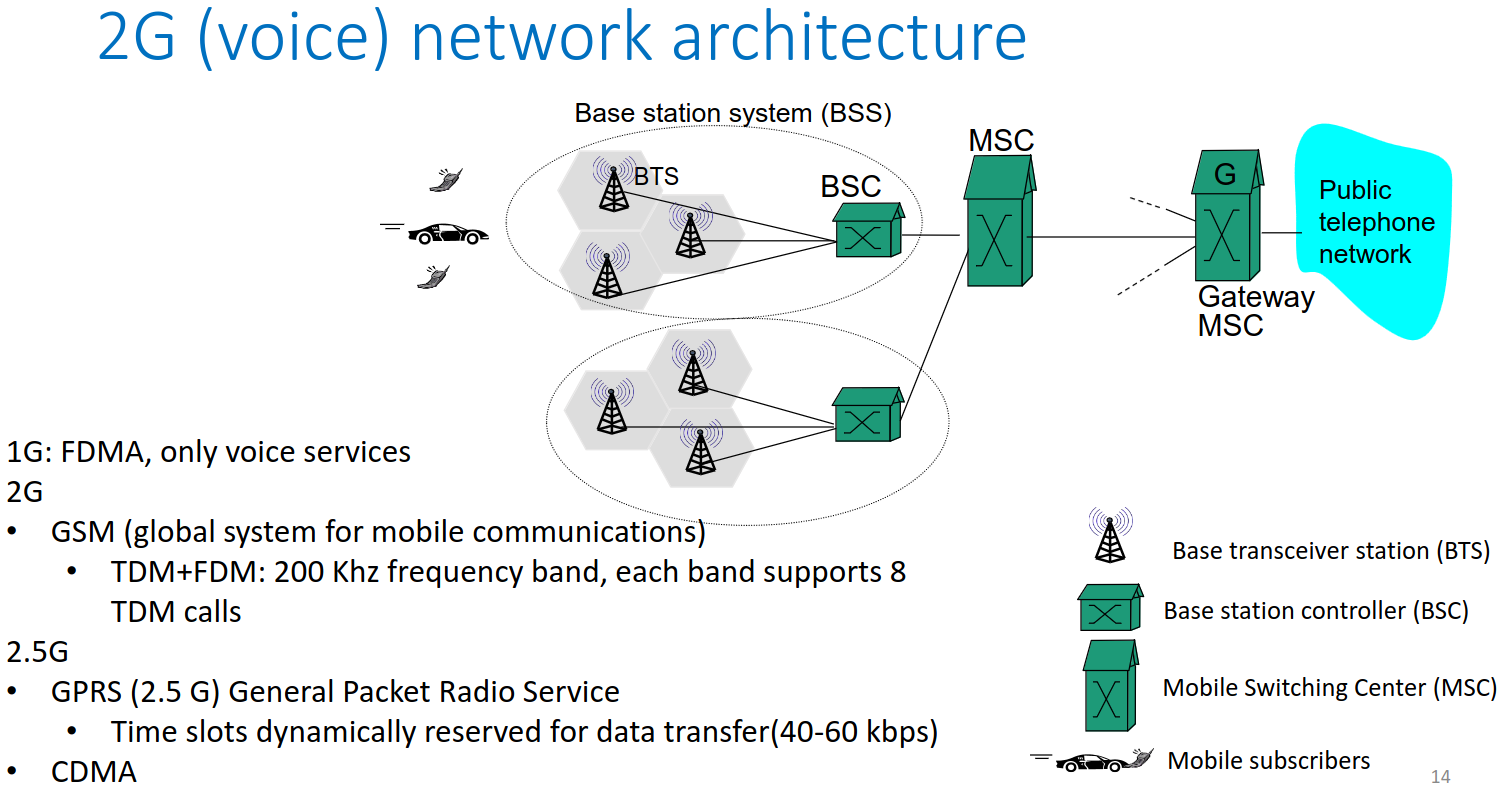
\includegraphics[width=0.45\columnwidth]{images/2g_architecture.png}
   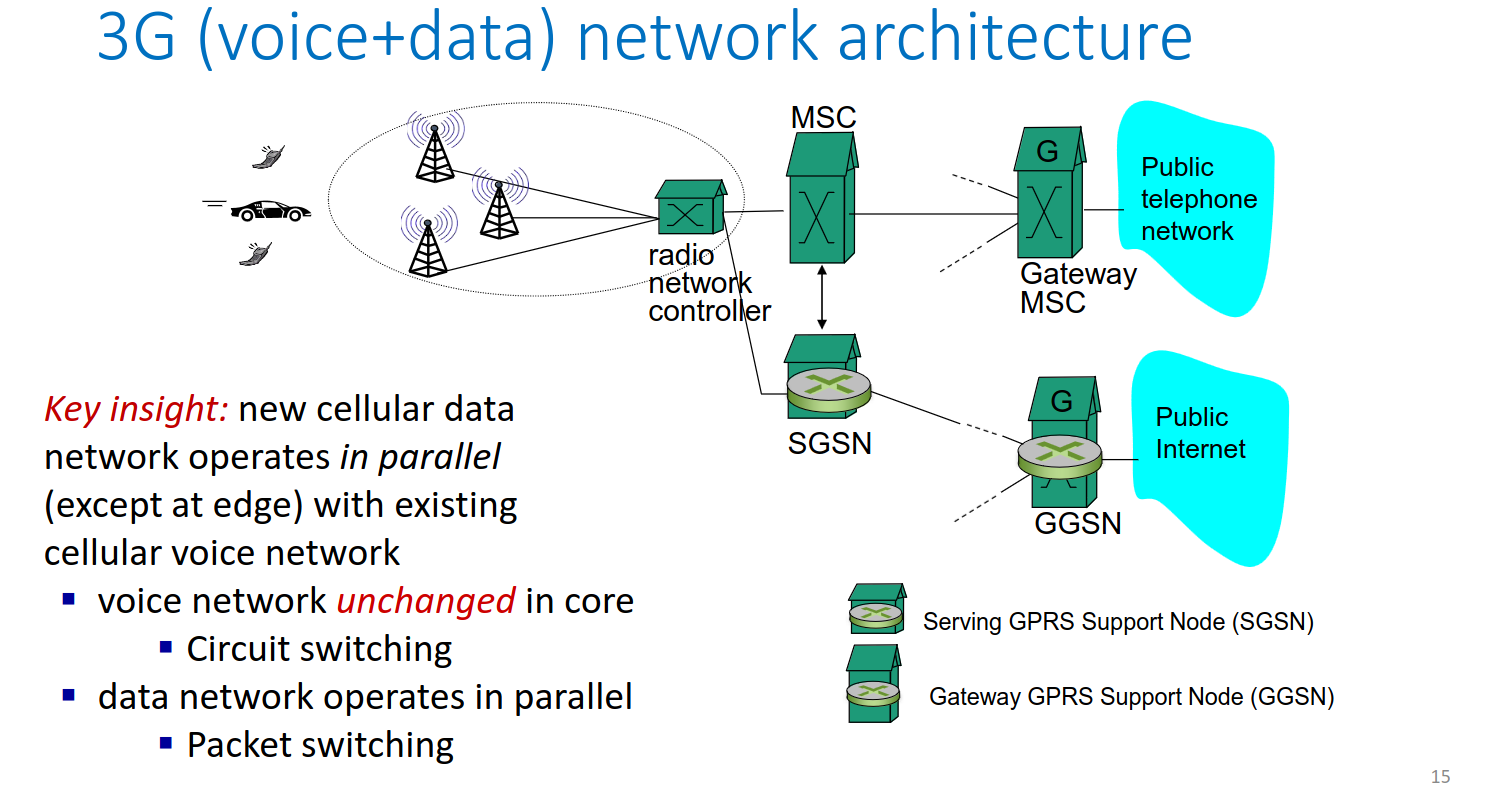
\includegraphics[width=0.45\columnwidth]{images/3g_architecture.png}\\
   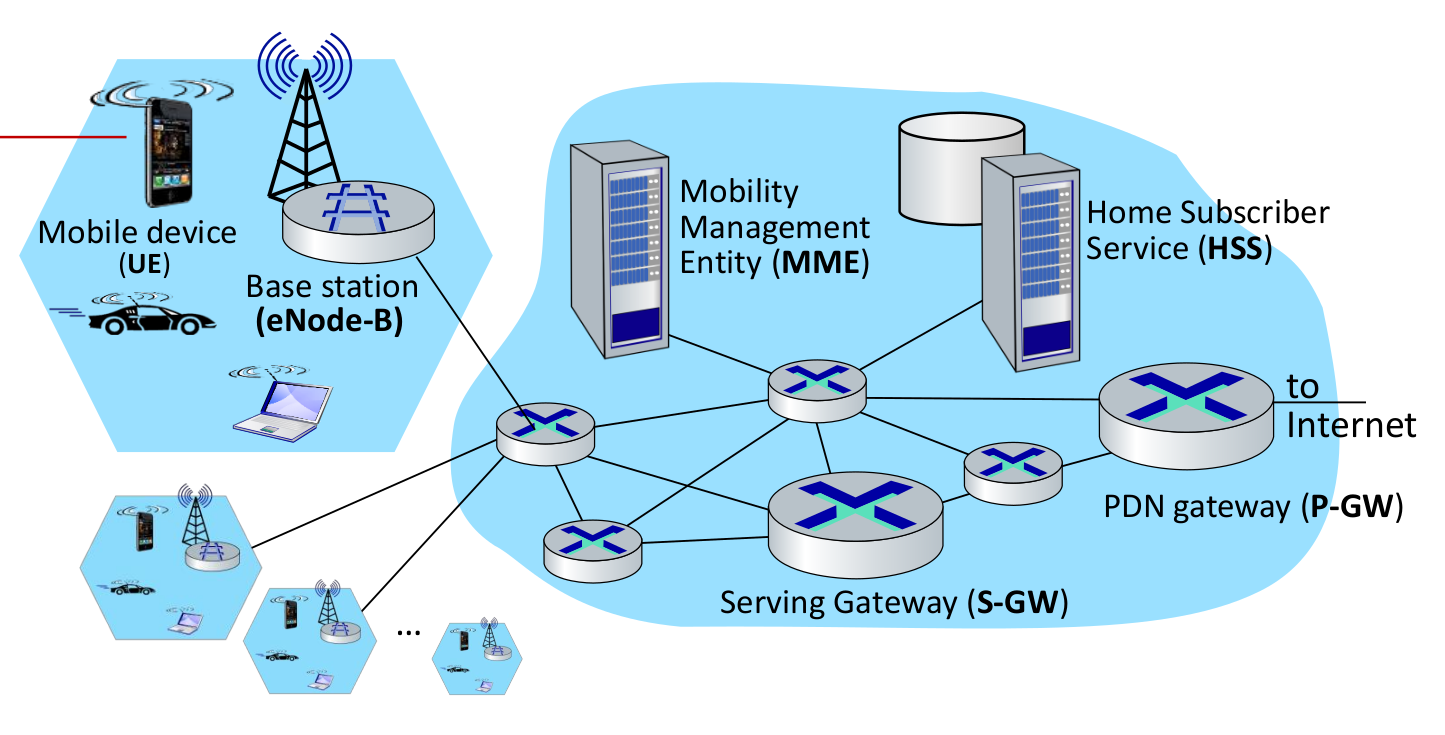
\includegraphics[width=0.45\columnwidth]{images/4g_architecture.png}
   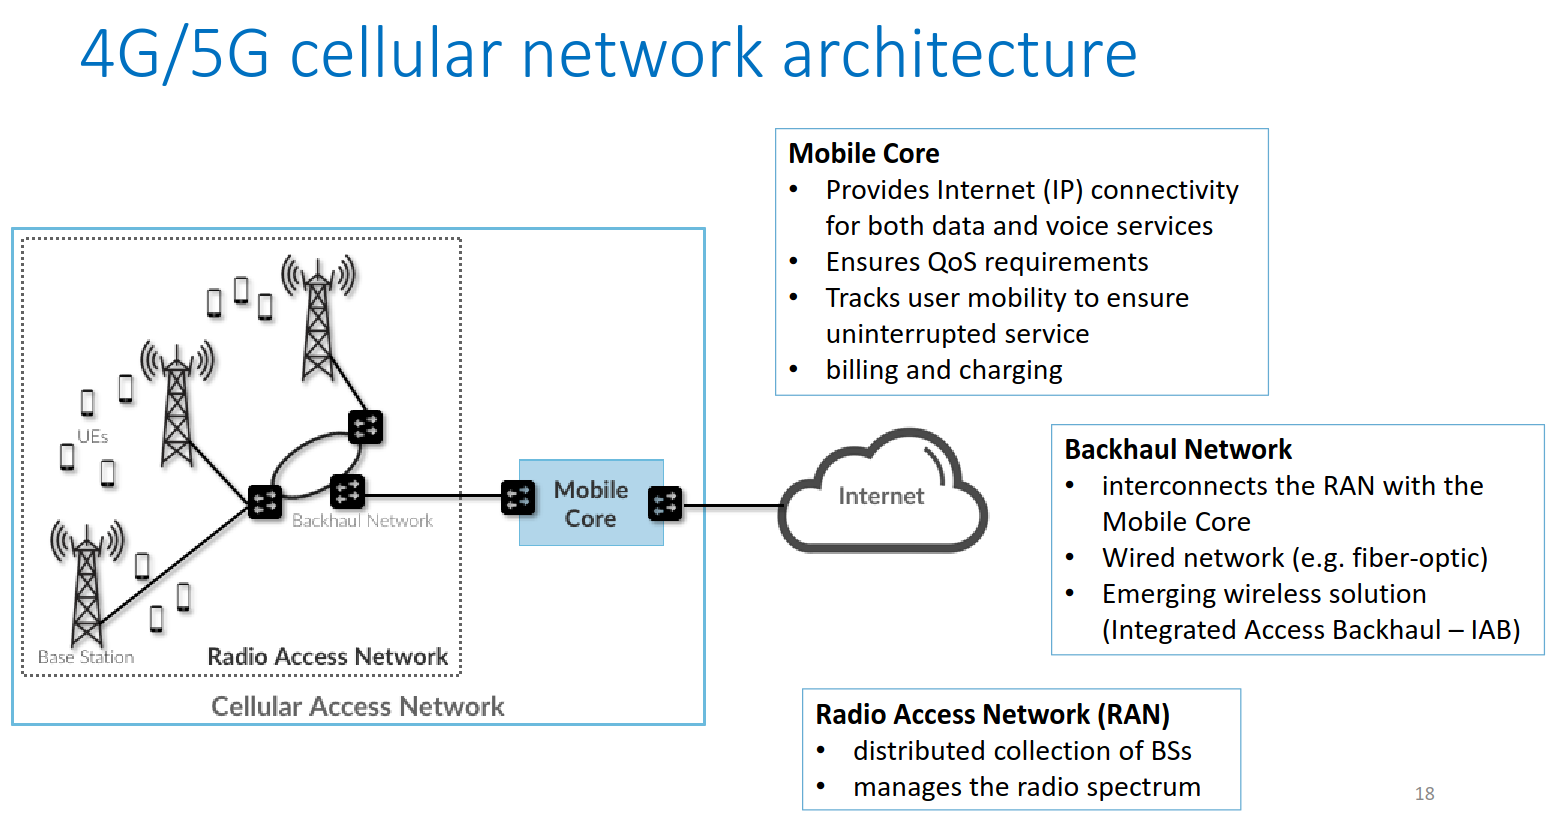
\includegraphics[width=0.45\columnwidth]{images/5g_architecture.png}

   \caption{Mobile Networks architectures}
   \label{fig:mobile_architectures}
\end{figure}

The key point in \textbf{3G} is the introduction of a data service, operating in parallel with voice network, which forced the important modifications to the architecture.

In \textbf{4G} also the voice traffic uses \textit{packet switching}, instead of circuit switching.

\framedt{Control vs Data plane}{
   \textbf{Control plane} includes routing protocols such as BGP and all the processes which handle and determine how data packets should be forwarded.
   
   \textbf{Data plane} instead handles the transport of host/application data, and performs the actually forwarding of packets.
   
   \textit{\footnotesize``Think of the control plane as being like the stoplights that operate at the intersections of a city. Meanwhile, the data plane (or the forwarding plane) is more like the cars that drive on the roads, stop at the intersections, and obey the stoplights''}
   \href{https://www.cloudflare.com/it-it/learning/network-layer/what-is-the-control-plane/}{Cloudflare Data/Control plane}
}


